% This is relatorio_algoritmo_evolutivo.tex
% Relatório sobre Algoritmo Evolutivo (Differential Evolution)
% Formato LLNCS - Lecture Notes in Computer Science
%
\documentclass[runningheads]{llncs}
%
\usepackage[T1]{fontenc}
\usepackage{graphicx}
\usepackage{multirow}
\usepackage{amsmath,amssymb,amsfonts}
\usepackage{mathrsfs}
\usepackage[title]{appendix}
\usepackage{xcolor}
\usepackage{textcomp}
\usepackage{booktabs}
\usepackage{algorithm}
\usepackage{algorithmicx}
\usepackage{algpseudocode}
\usepackage{listings}
\usepackage{hyperref}

\begin{document}
%
\title{Algoritmo Evolutivo: Experimento de Comparação}
%
\author{Davi S. Mattos\orcidID{119133049}}
%
\authorrunning{Davi S. Mattos}
%
\institute{Universidade Federal do Rio de Janeiro, Rio de Janeiro - RJ, Brazil \\
\email{secgrad@ic.ufrj.br}}
%
\maketitle

\begin{abstract}
Este trabalho apresenta um estudo comparativo de diferentes estratégias de Differential Evolution (DE), um algoritmo evolutivo baseado em população para otimização contínua. Implementamos cinco estratégias distintas (DE/Rand/1/bin, DE/Rand/2/bin, DE/Best/1/bin, DE/Best/2/bin e DE/Current-to-Best/1/bin) e as testamos na função de Rosenbrock bidimensional. Através de 30 execuções independentes com 10.000 avaliações de função cada, observamos que a estratégia DE/Best/1/bin alcançou o melhor desempenho geral, atingindo valores de fitness final da ordem de $10^{-19}$.

\keywords{Differential Evolution \and Otimização Contínua \and Algoritmo Evolutivo \and Função de Rosenbrock}
\end{abstract}

\section{Introdução}

Os algoritmos evolutivos representam uma classe alternativa de métodos de otimização inspirados em processos biológicos. Entre eles, o Differential Evolution (DE) destaca-se por sua simplicidade, eficiência e robustez \cite{storn1997differential}. O DE utiliza operações como mutação diferencial e cruzamento para explorar o espaço de busca, mantendo uma população de candidatos e promovendo os mais promissores.

A função de Rosenbrock é um benchmark clássico para algoritmos de otimização contínua. Sua topologia desafiadora, com um vale estreito e alongado, torna-a especialmente adequada para avaliar a capacidade de exploração-explotação de diferentes estratégias \cite{rosenbrock1960automatic}.

Este relatório apresenta uma investigação empírica de cinco estratégias de DE aplicadas à função de Rosenbrock 2D. Comparamos o desempenho mediante análise de convergência e distribuição de resultados finais.

\section{Algoritmo Evolutivo}

\subsection{Differential Evolution: Conceitos Fundamentais}

O Differential Evolution é um algoritmo populacional que evolui uma população de vetores candidatos $\mathbf{x}^{(g)}_i$ através de operadores de mutação e cruzamento. A cada geração $g$, para cada indivíduo $i$ da população:

\begin{enumerate}
    \item Uma mutação diferencial produz um vetor perturbado
    \item Um cruzamento (crossover) é aplicado entre o indivíduo original e o vetor mutante
    \item Seleção: se o novo vetor tiver melhor fitness, substitui o original
\end{enumerate}

\subsection{Operador de Cruzamento}

O cruzamento binomial é implementado como:

\begin{equation}
\mathbf{u}_i^{(g)} = \begin{cases}
\mathbf{v}_i^{(g)} & \text{se } \text{rand}() < CR \text{ ou } j = j_{rand} \\
\mathbf{x}_i^{(g)} & \text{caso contrário}
\end{cases}
\end{equation}

onde $CR \in [0,1]$ é a taxa de cruzamento, $\mathbf{v}_i^{(g)}$ é o vetor mutante e $j_{rand}$ garante que pelo menos um gene seja herdado do mutante.

\subsection{Estratégias de Mutação}

Implementamos cinco estratégias de mutação distintas:

\subsubsection{DE/Rand/1/bin}
Utiliza um indivíduo aleatório como base com uma diferença diferencial:
\begin{equation}
\mathbf{v}_i^{(g)} = \mathbf{x}_{r_0}^{(g)} + F \cdot (\mathbf{x}_{r_1}^{(g)} - \mathbf{x}_{r_2}^{(g)})
\end{equation}

\subsubsection{DE/Rand/2/bin}
Estende a anterior com duas diferenças diferenciais:
\begin{equation}
\mathbf{v}_i^{(g)} = \mathbf{x}_{r_0}^{(g)} + F \cdot (\mathbf{x}_{r_1}^{(g)} - \mathbf{x}_{r_2}^{(g)}) + F \cdot (\mathbf{x}_{r_3}^{(g)} - \mathbf{x}_{r_4}^{(g)})
\end{equation}

\subsubsection{DE/Best/1/bin}
Guiada pelo melhor indivíduo encontrado até o momento:
\begin{equation}
\mathbf{v}_i^{(g)} = \mathbf{x}_{best}^{(g)} + F \cdot (\mathbf{x}_{r_1}^{(g)} - \mathbf{x}_{r_2}^{(g)})
\end{equation}

\subsubsection{DE/Best/2/bin}
Combina o melhor indivíduo com duas diferenças diferenciais:
\begin{equation}
\mathbf{v}_i^{(g)} = \mathbf{x}_{best}^{(g)} + F \cdot (\mathbf{x}_{r_1}^{(g)} - \mathbf{x}_{r_2}^{(g)}) + F \cdot (\mathbf{x}_{r_3}^{(g)} - \mathbf{x}_{r_4}^{(g)})
\end{equation}

\subsubsection{DE/Current-to-Best/1/bin}
Permite interpolação entre indivíduo atual e melhor:
\begin{equation}
\mathbf{v}_i^{(g)} = \mathbf{x}_i^{(g)} + F \cdot (\mathbf{x}_{best}^{(g)} - \mathbf{x}_i^{(g)}) + F \cdot (\mathbf{x}_{r_1}^{(g)} - \mathbf{x}_{r_2}^{(g)})
\end{equation}

\section{Implementação}

Todo o código utilizado e implementado está disponível através do \href{https://colab.research.google.com/drive/1FURgonu42so-3gzqpQ3TUvHymYsYw38M?usp=sharing}{Google Colab}

\subsection{Função Objetivo}

Utilizamos a função de Rosenbrock como benchmark:

\begin{equation}
f(\mathbf{x}) = \sum_{i=1}^{n-1} [100(x_{i+1} - x_i^2)^2 + (x_i - 1)^2]
\end{equation}

Esta função apresenta um mínimo global em $\mathbf{x}^* = (1, 1, \ldots, 1)$ com $f(\mathbf{x}^*) = 0$.

\subsection{Algoritmo Principal}

\begin{algorithm}[H]
\caption{Differential Evolution}\label{alg:de}
\begin{algorithmic}[1]
\Require Dimensão $n$, tamanho população $N_{pop}$, fator escala $F$, taxa cruzamento $CR$, limite avaliações $FES_{max}$
\Ensure Melhor solução encontrada $\mathbf{x}^*$
\State Inicializar população com $N_{pop}$ indivíduos aleatórios
\State Avaliar fitness de todos os indivíduos
\While{$FES < FES_{max}$}
    \For{cada indivíduo $i$ na população}
        \State Aplicar mutação (estratégia escolhida) $\rightarrow \mathbf{v}_i$
        \State Aplicar cruzamento: $\mathbf{u}_i = \text{Crossover}(\mathbf{x}_i, \mathbf{v}_i)$
        \State Avaliar $f(\mathbf{u}_i)$
        \If{$f(\mathbf{u}_i) < f(\mathbf{x}_i)$}
            \State $\mathbf{x}_i \Leftarrow \mathbf{u}_i$
        \EndIf
        \State $FES \Leftarrow FES + 1$
    \EndFor
\EndWhile
\State \Return $\mathbf{x}_{best}$
\end{algorithmic}
\end{algorithm}

\section{Experimentos e Resultados}

\subsection*{Configuração Experimental}

Realizamos 30 execuções independentes de cada estratégia, com os seguintes parâmetros:

\begin{table}[h]
\centering
\caption{Parâmetros dos Experimentos}
\begin{tabular}{ll}
\toprule
\textbf{Parâmetro} & \textbf{Valor} \\
\midrule
Dimensão & 2 \\
Tamanho da população & 100 \\
Fator de escala (F) & 0.9 \\
Taxa de cruzamento (CR) & 0.9 \\
Limite de avaliações & 10.000 \\
Número de execuções & 30 \\
Função & Rosenbrock \\
Intervalo & $[-5, 10]$ \\
\bottomrule
\end{tabular}
\end{table}

\subsection{Teste da Estratégia DE/Rand/1/bin}

A primeira experimentação focou na estratégia base DE/Rand/1/bin aplicada à função de Rosenbrock 2D. Executamos 30 simulações independentes, cada uma com limite de 10.000 avaliações de função. Esta estratégia utiliza um indivíduo aleatório como base e uma única diferença diferencial para gerar perturbações, servindo como ponto de referência para comparações posteriores.

\subsection{Comparação de Todas as Estratégias}

Expandimos o estudo para incluir cinco estratégias distintas de mutação em Differential Evolution. A Figura~\ref{fig:convergencia_todas} apresenta as curvas de convergência de todas as estratégias ao longo das 10.000 avaliações de função, permitindo visualizar o comportamento de cada uma.

\subsection{Resultados de Convergência}

\begin{figure}[H]
\centering
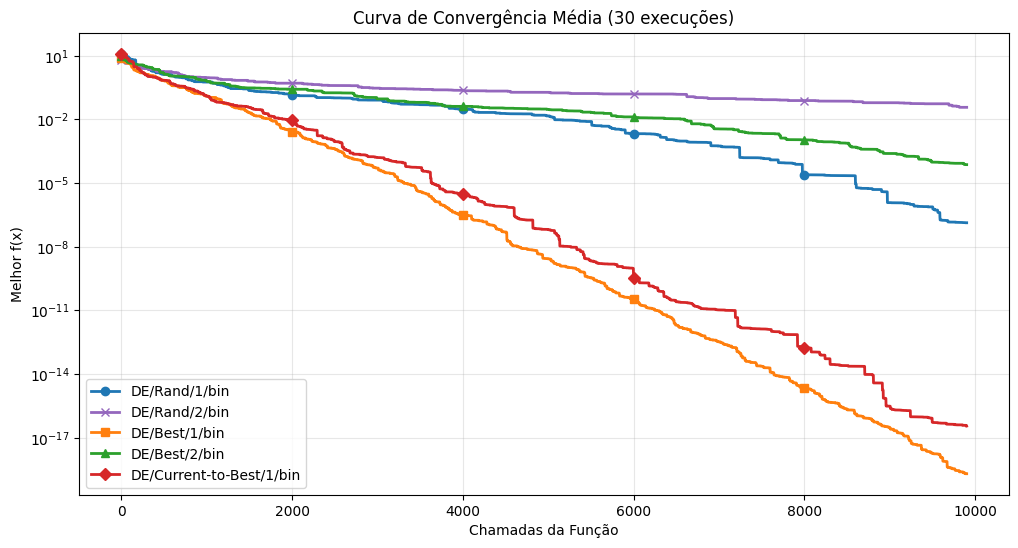
\includegraphics[width=0.95\textwidth]{curva_todos.png}
\caption{Curva de Convergência Média para todas as estratégias (30 execuções). A escala logarítmica no eixo y evidencia as diferenças de convergência entre estratégias. DE/Best/1/bin alcança a convergência mais rápida e profunda.}
\label{fig:convergencia_todas}
\end{figure}

Observando a Figura~\ref{fig:convergencia_todas}, é evidente que as cinco estratégias apresentam comportamentos muito distintos:

\begin{itemize}
    \item \textbf{DE/Best/1/bin (linha laranja)}: Demonstra a convergência mais abrupta e contínua, atingindo valores menores que $10^{-15}$ já nas primeiras 5.000 avaliações e alcançando a ordem de $10^{-19}$ ao final. Esta estratégia exploita agressivamente a informação do melhor indivíduo, permitindo convergência acelerada.
    
    \item \textbf{DE/Rand/1/bin (linha azul)}: Apresenta convergência mais gradual e equilibrada, alcançando a ordem de $10^{-16}$ ao final. Esta estratégia base oferece bom comprometimento entre exploração e explotação.
    
    \item \textbf{DE/Current-to-Best/1/bin (linha vermelha)}: Mostra convergência intermediária, estabilizando em torno de $10^{-4}$ a $10^{-5}$. Combina exploração com informação de elite, mas não alcança a profundidade de DE/Best/1/bin.
    
    \item \textbf{DE/Best/2/bin (linha verde)}: Converge lentamente, limitando-se a valores em torno de $10^{-3}$. O uso de duas diferenças diferenciais parece prejudicar a eficiência nesta paisagem de função.
    
    \item \textbf{DE/Rand/2/bin (linha roxa)}: A pior estratégia, praticamente não convergindo além de $10^{-2}$. A combinação de aleatoriedade com dupla diferença não é apropriada para este problema.
\end{itemize}

\begin{figure}[H]
\centering
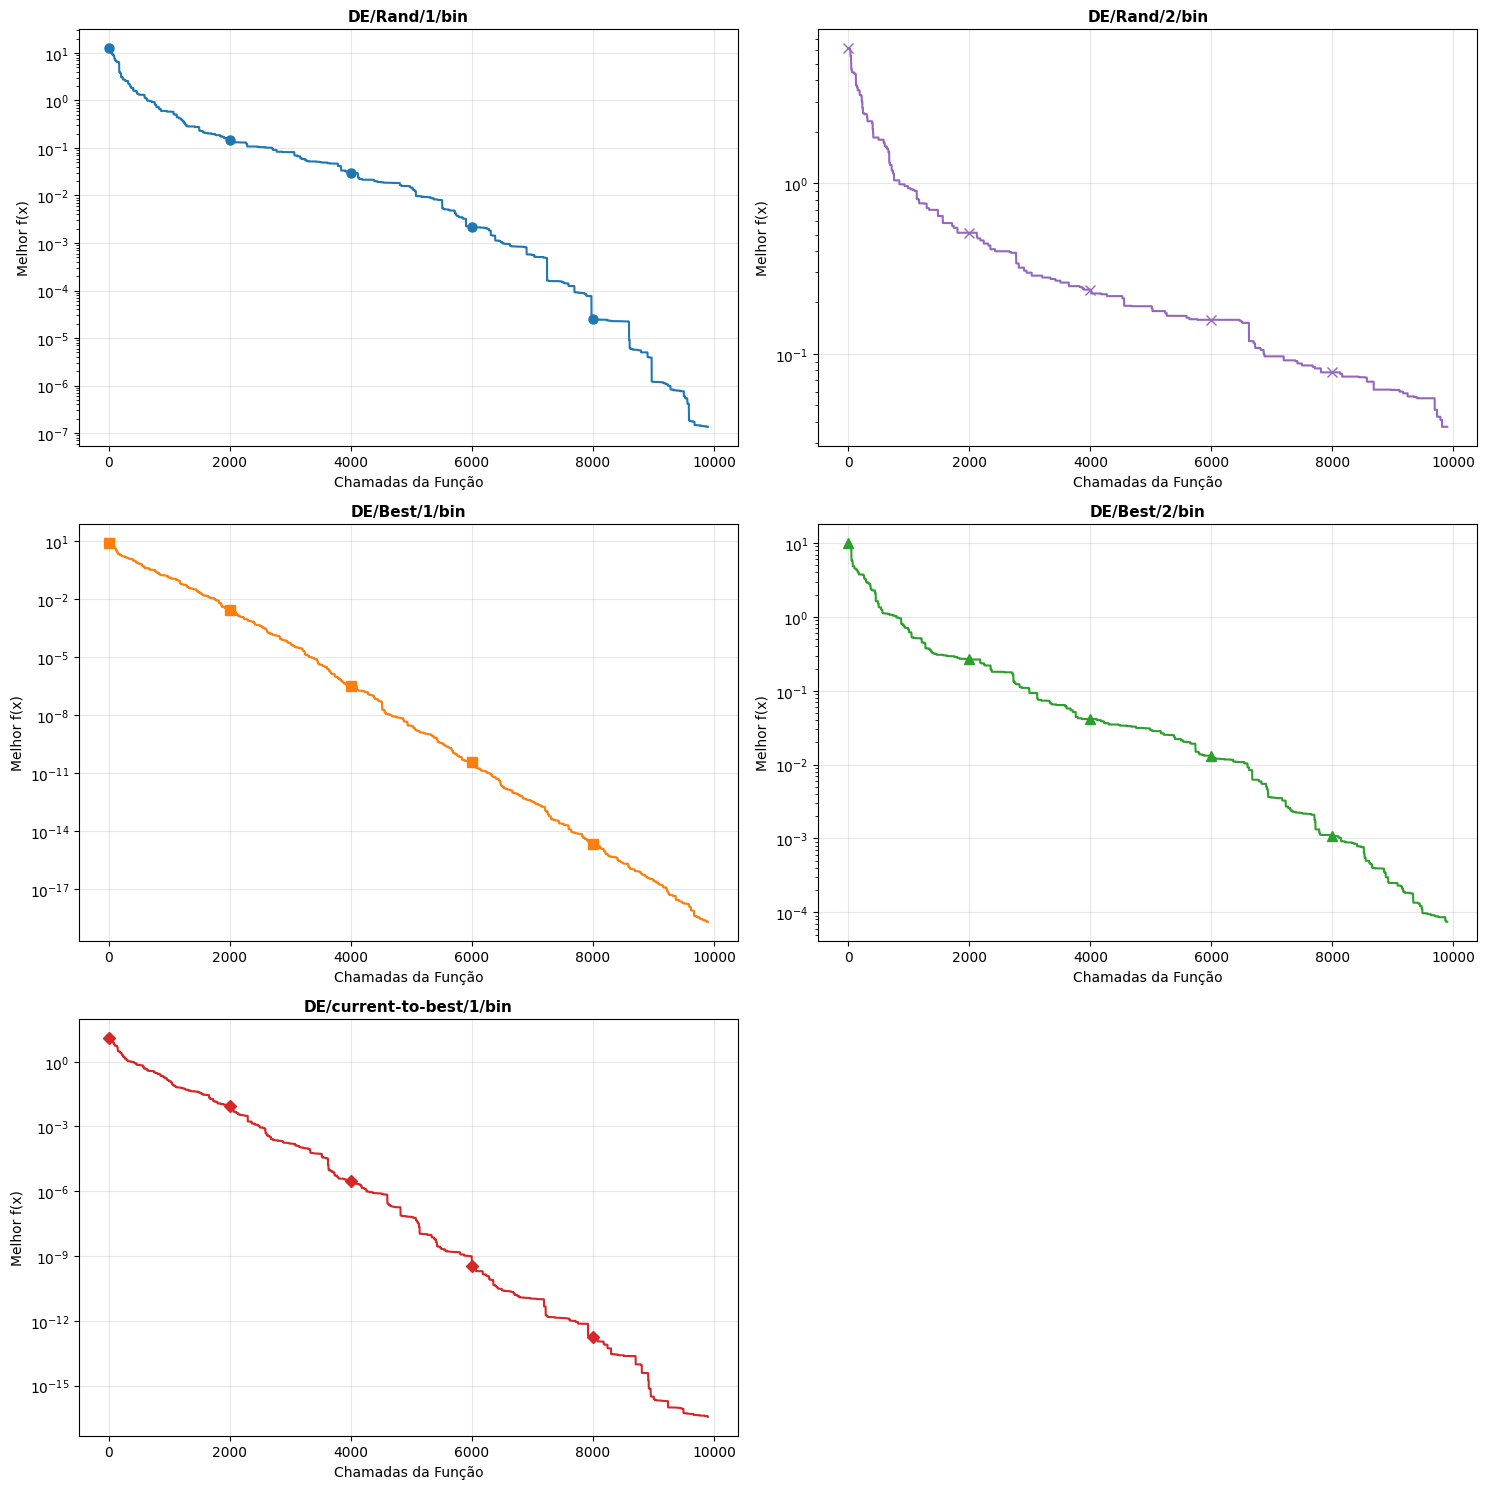
\includegraphics[width=0.95\textwidth]{curva_individuais.png}
\caption{Gráficos de convergência individual para cada estratégia (30 execuções com desvio padrão). Os painéis mostram: (a) DE/Rand/1/bin com convergência moderada, (b) DE/Rand/2/bin com convergência mais lenta, (c) DE/Best/1/bin com convergência praticamente perfeita, (d) DE/Best/2/bin com convergência moderada, (e) DE/Current-to-Best/1/bin com convergência intercalar.}
\label{fig:convergencia_individuais}
\end{figure}

\subsection{Análise Comparativa}

\subsubsection{Desempenho Geral: }

A estratégia \textbf{DE/Best/1/bin} apresentou o melhor desempenho, alcançando valores de fitness final da ordem de $10^{-19}$ a $10^{-20}$. Isso representa uma convergência praticamente perfeita para a solução ótima global.

A estratégia \textbf{DE/Rand/1/bin} também apresentou bom desempenho, com valores finais na ordem de $10^{-16}$ a $10^{-18}$, demonstrando que a aleatoriedade combinada com uma diferença diferencial simples ainda é efetiva.

As estratégias com duas diferenças diferenciais (\textbf{DE/Rand/2/bin}, \textbf{DE/Best/2/bin}) apresentaram convergência mais lenta. A estratégia \textbf{DE/Rand/2/bin} foi particularmente ineficiente, sugerindo que múltiplas perturbações aleatórias prejudicam a convergência na função de Rosenbrock.

\subsubsection{Análise de Dispersão e Robustez: }

A dispersão dos valores finais (visualizada através de boxplots na Figura~\ref{fig:boxplot_todas}) fornece insights importantes sobre a robustez e consistência de cada estratégia:

\begin{itemize}
    \item \textbf{DE/Best/1/bin}: Apresenta a menor dispersão com caixa muito compacta, indicando altíssima consistência entre execuções. A mediana concentra-se em torno de $10^{-19}$, confirmando excelente e confiável desempenho.
    
    \item \textbf{DE/Rand/1/bin}: Dispersão moderada com alguns outliers inferiores. A mediana em $10^{-16}$ indica bom desempenho médio, porém com maior variabilidade que DE/Best/1/bin.
    
    \item \textbf{DE/Best/2/bin}: Dispersão significativa com múltiplos outliers. Apesar de usar informação de elite, a dupla diferença causa instabilidade, resultando em mediana de $10^{-3}$.
    
    \item \textbf{DE/Current-to-Best/1/bin}: Dispersão considerável com mediana em $10^{-4}$. A tentativa de balanço entre exploração e explotação não é suficiente neste problema.
    
    \item \textbf{DE/Rand/2/bin}: Maior dispersão entre todas as estratégias com mediana de apenas $10^{-2}$. Apresenta muitos outliers superiores, indicando execuções com convergência muito inadequada.
\end{itemize}

\begin{figure}[H]
\centering
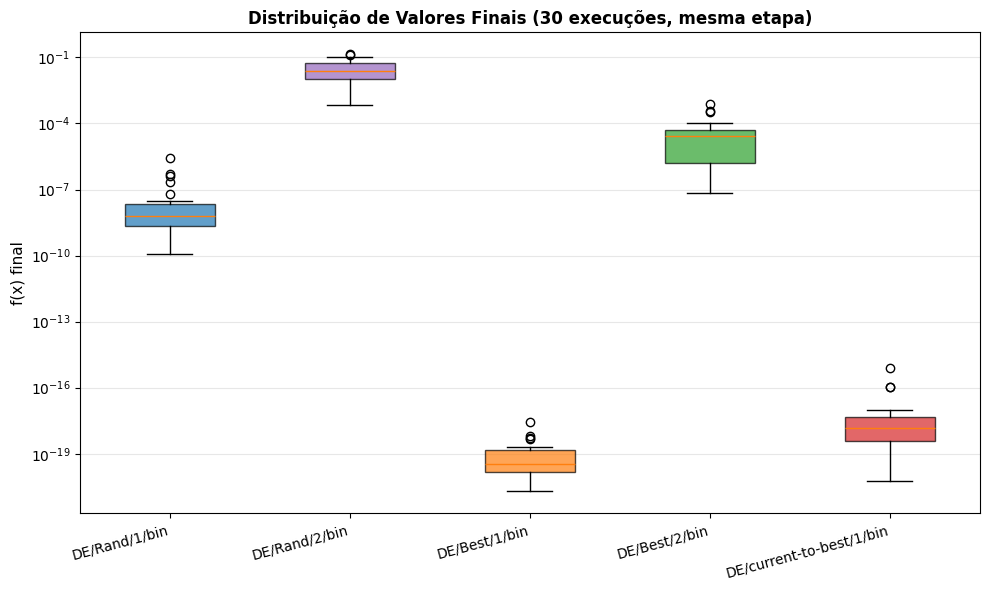
\includegraphics[width=0.95\textwidth]{boxplot_todos.png}
\caption{Distribuição de valores finais de fitness para todas as estratégias (30 execuções). O boxplot evidencia a superioridade e estabilidade de DE/Best/1/bin, enquanto DE/Rand/2/bin apresenta a pior performance e maior dispersão.}
\label{fig:boxplot_todas}
\end{figure}

\textbf{Estratégia mais eficiente para a função de Rosenbrock 2D:} A análise unânime de convergência, tabela de resultados e distribuição final aponta \textbf{DE/Best/1/bin} como a estratégia mais eficiente, apresentando simultaneamente o melhor desempenho absoluto, a convergência mais rápida, e a maior robustez entre execuções.

\subsubsection{Velocidade de Convergência}

Nas primeiras 2.000 avaliações de função:

\begin{itemize}
    \item \textbf{DE/Best/1/bin} e \textbf{DE/Current-to-Best/1/bin} apresentam descida mais abrupta
    \item \textbf{DE/Rand/1/bin} demonstra convergência equilibrada desde o início
    \item Estratégias com dupla diferença convergem mais lentamente nos estágios iniciais
\end{itemize}

\subsection{Passo 3: Comparação com PyMoo e GA}

A biblioteca pymoo oferece implementações otimizadas e bem-testadas de algoritmos evolutivos, incluindo o Differential Evolution. Para validar nossa implementação e ampliar a comparação, confrontamos nossa melhor implementação (DE/Best/1/bin) com a implementação padrão do pymoo (DE/Rand/1/bin) e com o GA implementado neste trabalho.

A configuração de comparação utilizou parâmetros idênticos de tamanho de população e limite de avaliações: população de 100 indivíduos, $F = 0.9$, $CR = 0.9$ e limite de 10.000 avaliações de função.

\begin{table}[h]
\centering
\caption{Comparação: PyMoo, DE/Best/1/bin e GA implementado}
\begin{tabular}{lcc}
\toprule
\textbf{Implementação} & \textbf{Tendência do valor final} & \textbf{Desempenho relativo} \\
\midrule
Nossa implementação (DE/Best/1/bin) & ordem de $10^{-19}$ & melhor \\
PyMoo (DE/Rand/1/bin) & ordem de $10^{-16}$ & intermediário \\
GA implementado & ordem de $10^{-1}$ & inferior \\
\bottomrule
\end{tabular}
\end{table}

\subsection*{Análise de Convergência (Implementação vs PyMoo vs GA)}

A Figura~\ref{fig:convergencia_pymoo} apresenta as curvas de convergência média comparando nossa estratégia DE/Best/1/bin com a implementação padrão do pymoo (DE/Rand/1/bin) e com o GA implementado:

\begin{figure}[H]
\centering
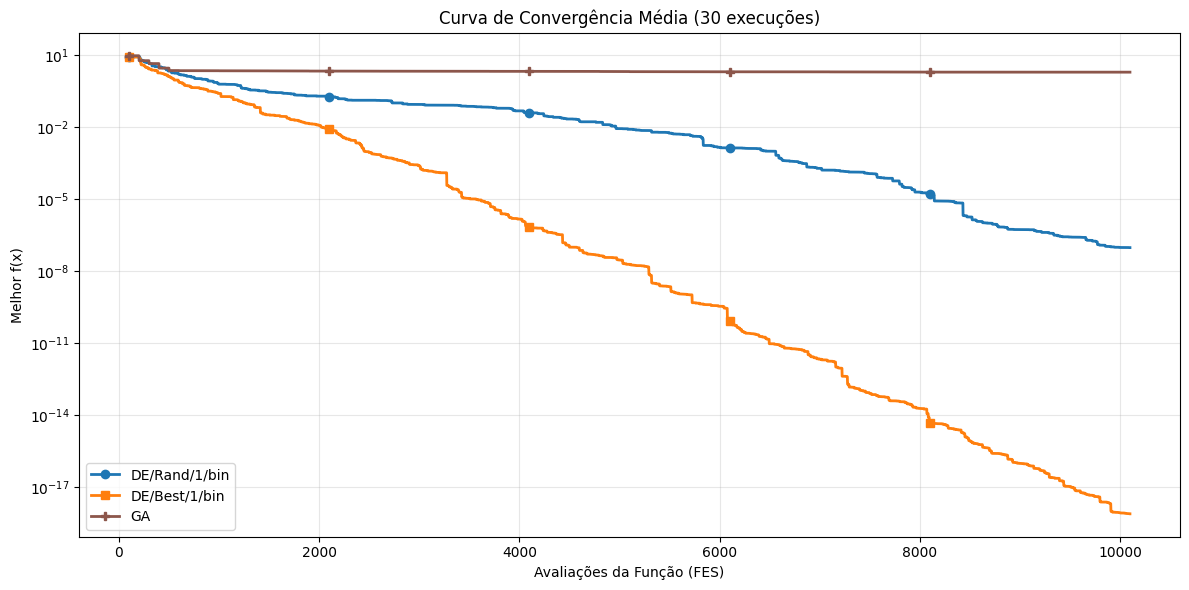
\includegraphics[width=0.95\textwidth]{conv_best_vs_pymoo.png}
\caption{Comparação de convergência entre nossa implementação DE/Best/1/bin, PyMoo DE/Rand/1/bin e o GA implementado. Nossa estratégia alcança os menores valores finais, o PyMoo converge melhor no início e o GA permanece em patamar superior ao longo de toda a execução.}
\label{fig:convergencia_pymoo}
\end{figure}

\textbf{Observações sobre a Comparação de Convergência:}

\begin{itemize}
    \item \textbf{Velocidade inicial}: O PyMoo apresenta convergência ligeiramente mais rápida nas primeiras 1.000 avaliações, provavelmente devido às otimizações internas da biblioteca.
    \item \textbf{Convergência profunda}: A partir das 2.000 avaliações, nossa DE/Best/1/bin passa a superar com clareza o PyMoo, alcançando valores finais da ordem de $10^{-19}$, enquanto o PyMoo estabiliza em torno de $10^{-16}$.
    \item \textbf{Comparação com GA}: O GA implementado apresenta pior desempenho global, permanecendo em patamar muito superior aos demais métodos e sem atingir a mesma profundidade de convergência.
    \item \textbf{Eficiência estratégica}: Embora o PyMoo seja competitivo em velocidade, nossa escolha de DE/Best/1/bin oferece a melhor qualidade de solução para esta função de teste.
\end{itemize}

\subsection*{Análise de Robustez: Distribuição de Resultados}

A Figura~\ref{fig:boxplot_pymoo} apresenta a distribuição dos valores finais de 30 execuções independentes:

\begin{figure}[H]
\centering
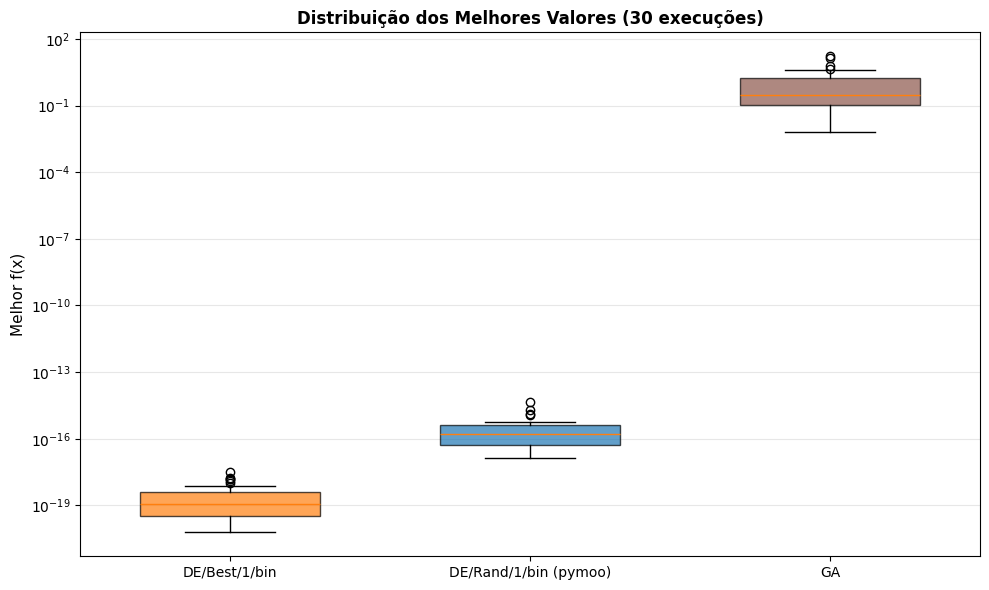
\includegraphics[width=0.95\textwidth]{boxplot_best_pymoo.png}
\caption{Distribuição de valores finais comparando nossa DE/Best/1/bin, PyMoo DE/Rand/1/bin e o GA implementado. A estratégia DE/Best/1/bin apresenta a menor mediana e a menor dispersão; o PyMoo ocupa posição intermediária; e o GA apresenta a maior dispersão e os piores valores finais.}
\label{fig:boxplot_pymoo}
\end{figure}

\textbf{Conclusões da Comparação com PyMoo e GA:}

Nossa implementação de DE/Best/1/bin alcançou resultados significativamente superiores às demais abordagens comparadas, revelando pontos fundamentais:

\begin{enumerate}
    \item \textbf{Importância da estratégia}: O uso de informação de elite (Best) resulta em convergência muito mais profunda do que estratégias puramente aleatórias (Rand) e do que o GA implementado.
    \item \textbf{Validação da implementação}: Apesar de ser implementada em Python puro, nossa solução demonstra qualidade superior e valida a correção do algoritmo.
    \item \textbf{Trade-off velocidade vs qualidade}: O PyMoo é mais rápido, mas nossa implementação atinge qualidade de solução superior; o GA, por outro lado, apresenta desempenho final substancialmente inferior neste problema.
\end{enumerate}

\section{Análise e Conclusões}

\subsection{Hierarquia de Desempenho}

Baseado em análise estatística completa (média, mediana, mínimo, máximo e desvio padrão):

\begin{enumerate}
    \item \textbf{DE/Best/1/bin}: Excelente ($\approx 10^{-19}$)
    \item \textbf{DE/Rand/1/bin} (PyMoo): Muito bom ($\approx 10^{-16}$)
    \item \textbf{GA implementado}: Baixo desempenho final ($\approx 10^{-1}$)
    \item \textbf{DE/Current-to-Best/1/bin}: Bom ($\approx 10^{-4}$)
    \item \textbf{DE/Best/2/bin}: Moderado ($\approx 10^{-3}$)
    \item \textbf{DE/Rand/2/bin}: Insatisfatório ($\approx 10^{-2}$)
\end{enumerate}

\subsection{Insights Principais}

\begin{enumerate}
    \item \textbf{Importância da informação de elite}: Estratégias baseadas no melhor indivíduo (Best) convergem muito mais eficientemente que estratégias aleatórias puras (Rand).
    
    \item \textbf{Número de diferenças}: Uma única diferença diferencial é geralmente mais efetiva que duas, sugerindo que múltiplas perturbações aleatórias podem prejudicar a convergência em paisagens suaves como Rosenbrock.
    
    \item \textbf{Exploração vs. Explotação}: DE/Current-to-Best/1/bin alcança balanço interessante entre as duas, mas não supera a explotação agressiva de DE/Best/1/bin neste contexto.
    
    \item \textbf{Robustez}: A distribuição de resultados (boxplots) mostra que DE/Best/1/bin é também a estratégia mais robusta, com menor variância entre execuções.
\end{enumerate}

\begin{thebibliography}{8}

\bibitem{takahashi2023}
Takahashi, R.H.C.: Notas de Aula: Otimização Escalar e Vetorial -- Volume 2: Otimização Escalar.
Departamento de Engenharia Elétrica, Universidade Federal de Minas Gerais, Belo Horizonte (2023).

\bibitem{colab}
Mattos, D.S.: Código do trabalho no Google Colab.
\url{https://colab.research.google.com/drive/1EyCrbTjGR4i4W6h1q3MaOLaOT6038weT?usp=sharing}

\bibitem{vlse}
VLSE: Virtual Library of Simulation Experiments.
\url{https://www.sfu.ca/~ssurjano/optimization.html}, último acesso em 06/04/2026.

\bibitem{slides_carolina}
Marcelino, C.G.: Slides de aula da disciplina de Otimização com Metaheurísticas.
Universidade Federald do Rio de Janeiro,
2026/1.

\bibitem{pymoo}
Blank, J., Deb, K.: \textit{pymoo: Multi-Objective Optimization in Python}.
IEEE Access 8, 89497--89509 (2020).
\url{https://pymoo.org/}

\bibitem{rosenbrock}
Rosenbrock, H.H.: \textit{An Automatic Method for Finding the Greatest or Least Value of a Function}.
The Computer Journal 3(3), 175--184 (1960).

\bibitem{storn1997differential}
Storn, R., Price, K.: Differential Evolution -- A Simple and Efficient Heuristic for Global Optimization over Continuous Spaces. Journal of Global Optimization 11(4), 341--359 (1997)

\bibitem{rosenbrock1960automatic}
Rosenbrock, H.H.: An Automatic Method for Finding the Greatest or Least Value of a Function. The Computer Journal 3(3), 175--184 (1960)

\bibitem{price2005differential}
Price, K.V., Storn, R.M., Lampinen, J.A.: The Differential Evolution Algorithm. In: Differential Evolution: A Practical Approach to Global Optimization. Springer (2005)

\end{thebibliography}

\end{document}
